\documentclass[10pt,twocolumn,letterpaper]{article}

\usepackage{cvpr}
\usepackage{times}
\usepackage{epsfig}
\usepackage{graphicx}
\usepackage{amsmath}
\usepackage{amssymb}
\usepackage{multirow}
\usepackage{textcomp}

% Include other packages here, before hyperref.

% If you comment hyperref and then uncomment it, you should delete
% egpaper.aux before re-running latex.  (Or just hit 'q' on the first latex
% run, let it finish, and you should be clear).
\usepackage[breaklinks=true,bookmarks=false]{hyperref}

%\cvprfinalcopy % *** Uncomment this line for the final submission

\def\cvprPaperID{7347} % *** Enter the CVPR Paper ID here
\def\httilde{\mbox{\tt\raisebox{-.5ex}{\symbol{126}}}}

% Pages are numbered in submission mode, and unnumbered in camera-ready
\ifcvprfinal\pagestyle{empty}\fi
\setcounter{page}{1}
\begin{document}

%%%%%%%%% TITLE
\title{M-Protein Diagnostics Using Generative Active Learning}


\author{Hanyu Li\\
Department of Physics\\
Tsinghua University\\
{\tt\small l-hy16@mails.tsinghua.edu.cn}
% For a paper whose authors are all at the same institution,
% omit the following lines up until the closing ``}''.
% Additional authors and addresses can be added with ``\and'',
% just like the second author.
% To save space, use either the email address or home page, not both
\and
Junsong Yuan\\
Department of Computer Science and Engineering\\
University at Buffalo\\
{\tt\small jsyuan@buffalo.edu}
}

\maketitle
%\thispagestyle{empty}

%%%%%%%%% ABSTRACT
\begin{abstract}
    With comparatively less labeled data and high labeling cost, most of the medical involved tasks can not be directly tackled by state of art machine learning approaches for their lack of large carefully labeled datasets. Our paper is based on the a dataset of immunofixation electrophoresis(IFE) images used in the M-Protein diagnostics that has no annotation. In order to make the diagnostics process more efficient, our paper try to train a binary classifier(normal or not) with only few data instance labeled by human experts and all other unlabeled data. We do the semi-supervised training by combining active learning with generative models. In our proposed method, we do these things iteratively: first we find the most uncertain data instances in the latent space of the generative model using the classifier; then we generate synthetic IFE images for human oracle to annotate; afterwards we add these labeled data back in the training set of the classifier. In addition, according to prior knowledge of the IFE images, we propose a specific explainable generative model based on Gaussian mixture model(GMM) that is only effective in this dataset, and compare the result of it with universal effective generative model like GAN and VAE. In order to figure out the best representation of this dataset, we conduct extensive experiments to demonstrate the difference between applied generative models, evaluate the effect they make on active learning quantitavely, and explore the reason behind the results.
\end{abstract}

%%%%%%%%% BODY TEXT
\section{Introduction}

\par As deep models achieve astonishing results in almost every machine learning tasks, some unavoidable problems such as the need for large carefully labeled dataset has troubled researchers from the start. Part of the reason behind the tremendous success in deep learning is the availability of large-scale labeled data\cite{sun2017revisiting}. Although data labeling companies and platforms claim that they can provide inexpensive yet high quality data\cite{buhrmester2011amazon}, achieving such datasets can be extremely costly or even unrealistic in the scenarios where labeling requires high professionality. For instance, some medical image tasks can not be labeled by people without systematic training. However, the small number of these experts has determined that large-scale dataset is difficult to biuld. Plus, they are probably already preoccupied. With the desire to fill this gap, our paper combines active learning and generative model to achieve relatively good results on small datasets.

For instance, a large dataset of medical images regarding M-Protein diagnostics is accessible. Nonetheless, each image comes with a diagnostics report without the trainable label that we desire. M-Protein stands for Myeloma protein, which can be identified by applying immunofixation electrophoresis(IFE) because its sharp monoclonal band in the image. Different categories of results may indicate MGUS, smouldering myeloma(sMM), or multiple myeloma(MM). It usually takes three doctors to examine the IFE image and reach the final conclusion. Therefore the process is highly time consuming. In real world scenarios, more than half of the electrophoresis results are obviously normal which do not need further concern. Although final decision should be made by doctors, if a classifier can provide an indicating result, then time can be significantly saved. Part of the proposed method can be implemented by manually constructed rules, so in the end, machine learning involved section is narrowed down to a binary classification(normal or abnormal) of one dimensional signal.

Due to the lack of explicit label, this is a classic semi-supervised learning task. Our paper tries to utilize the combination of active learning and generative model to tackle with this unlabeled dataset. Active learning is that a machine learning algorithm that can achieve greater accuracy with same amount labeled training instances if it is allowed to choose the data to be labeled from an unlabeled dataset \cite{settles2009active}. Thus, active learning techniques significantly reduce the amount of labor required compared to manually label all existing data. Deep generative models including GAN and VAE are currently purveiling in a variety of applications. Zhu and Bento made the first attempt\cite{Zhu2017GenerativeAA} to generate data for active learning process. Since then, a number of research have been conducted to find the most effective way to boost the active learning performance using generative models.

\begin{figure*}
    \begin{center}
    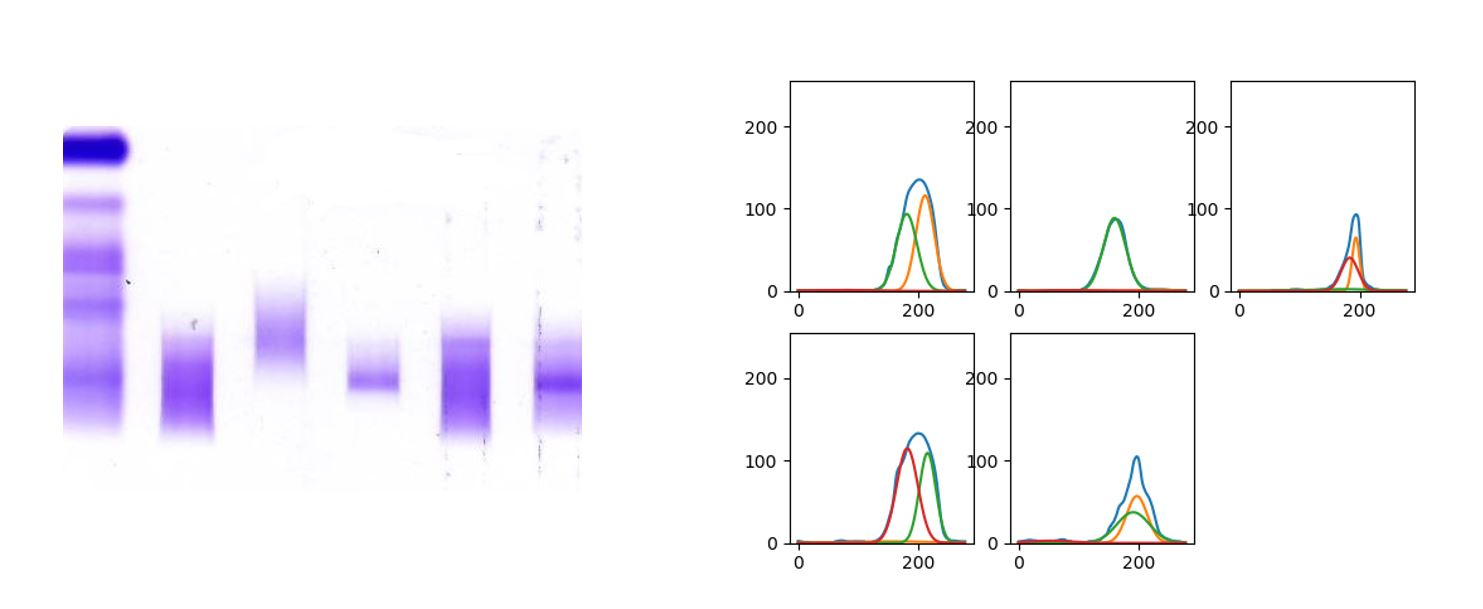
\includegraphics[width=0.9\linewidth]{fig_1.jpg}
    \end{center}
       \caption{An example of input image and its GMM decomposition. Blue curve is the density curve of the last five column(IFE columns), and other ones are the Gaussian components.}
    \label{fig:short}
\end{figure*}

Our paper also tries to utilize the combination of active learning and generative models to gain a task learner, but we made specific augmentations specifically for IFE column binary classification. By generating(decoding) synthetic IFE images based on latent space of the generative models, the model can query the least certain generated instances in the latent space, and thus improve the classifier in the latent space iteratively. In addition, according to prior knowledge of the IFE images, we propose a specific explainable generative model based on Gaussian mixture model(GMM) that is only effective in this dataset, and compare the result of it with universal effective generative model like GAN and VAE. We conduct extensive experiments to demonstrate the difference between applied generative models, evaluate the effect they make on active learning quantitavely, and try to find the reason behind it.

\subsection{Related Work}
Several techniques were widely used by researchers to tackle with small datasets and partially labeled datasets. For example, active learning\cite{settles2009active} tries to pick the most informative data to label so that models can learn better when the total number of labeled data is limited; generative methods\cite{kingma2014semi}\cite{springenberg2015unsupervised} wish to benifit target classifier using knowledge of data distribution learnt by generative models; data augmentation\cite{tanner1987calculation} enriches small dataset by generating new synthetic data; domain transfer\cite{pan2009survey} utilizes large, easily acquired datasets in different tasks or different settings to help the training of target learner. In this paper we mainly focus on active learning and generative methods.
\subsection{Active Learning}
In general, active learning has three main settings: membership query synthesis, stream-based selective sampling, and
pool-based active learning\cite{pan2009survey}. Among them the last one is mostly refered to. Pool-based active learning gather a large pool of unlabeled data and ranks their informativeness according to an acquisition function that may coevolve with the task learner in the training process. Various acquisition functions have been developed by researchers. For example, some acquisition function can be derived by maximising the uncertainty of the current learner(i.e. finding the most uncertain data in the pool). Another acquisition function maximises the Bayesian Active Learning by Disagreement(BALD)\cite{houlsby2011bayesian}. It can choose pool points that are expected to maximise the information gained about the model parameters through maximising the mutual information between predictions and model posterior. Nonetheless, active learning framework was specifically designed for datasets with rather small-scaled labeled data, and even after the iterative process of oracle labeling, the total number of trainable data is still significantly less than classic deep learning scenarios. Under such constraint, the task learner still suffer from overfitting problem when dealing with high-dimenisonal data. Only few researchers appled active learning on high-dimensional data, and to our best knowledge, almost all of them proposed special techniques\cite{Gal:2017:DBA:3305381.3305504}.
\subsection{Generative Methods}
Firstly proposed by Goodfellow \emph{et al.} in 2014, generative adversarial nets(GANs) \cite{goodfellow2014generative} drawn a lot attention in the field of computer vision, natual language processing, and etc. GAN plays a minimax game between the generator and the discriminator by training them simultaneously but with different goals. Previous researchers inspired by its adversarial structure developed a large amount of variations that can be applied to various kinds of tasks. Some of the most well-known variations of GAN includes WGAN\cite{arjovsky2017wasserstein} which stablizes training process and provide solution to mode collapse problem, CGAN\cite{mirza2014conditional} that firstly introduced models that can generate specific classes according to the label fed as part of the input, BiGAN\cite{donahue2016adversarial} that enables bidirectional transformation, VAEGAN\cite{larsen2015autoencoding} that connects GAN and VAE using a conjuncted generator/decoder, and so on. Variation auto encoder(VAE) on the other hand, tries to develop a generative model in a variation inference kind of way\cite{kingma2013auto}.It tries to capture the most important latent variables that determine how real data are formed. Although more robust to small perturbations in latent space, VAE tends to lose more graphic details(more blurry) when reconstructing the input data compared to GAN due to its pixel-wise reconstruction loss. 
\subsection{Generative Active Learning}
Conventional pool-based active learning method draws data to be labeled from the large unlabeled data pool. However, data in the unlabeled dataset are spread all over the data space. Hence, after exhausting the most informative data, the acquisition function will begin to query less informative data later on in the training process. However, if queried data are all synthesized(i.e. generated), its informativeness will not degrade over time. Moreover, given that the generative model fully captured the true distribution of data, it can generate informative data whose mode is not fully covered in the original dataset\cite{Zhu2017GenerativeAA}. Also, with promising conditional generative model like ACGAN, researchers came up with several models that free active learning from low dimensional data since unlimited labeled data can be generated\cite{kong2019active}. This great advantage comes with high risks though. Active learning demands data with sufficient information. In other words, generated data should yield high uncertainty. Thus, automatically labeled generative models suffer from the trade off between informativeness and safety of data. More common methods are to do active learning process in the latent variable space of the generative model. Huijser and Gemert proposed a novel boundary annotation approach to train a classifier in the latent space\cite{huijser2017active}. Every chosen data point in the latent space will determine a straight line which is perpendicular to the decision hyperplane, on which they pick points with equal distance. According to the results of the boundary location in these points, they shift the decision hyperplane so that it goes through the boundary data point. In another work, Tran \emph{et al.} modified iterative Bayesian data augmentation(BDA) framework using active learning and proposed VAE ACGAN model to tackle with the problem of BDA that it tends to generate less informative augmented data\cite{tran2019bayesian}.

  
\section{Preliminaries}
The entire defination of the task can be illustrated as below. Every IFE image consists of five columns of one dimensional signal with length of 300. Among them the first three column represents the heavy chain G, A, M, and the last two is the light chain $\kappa$, and $\lambda$. According to an IFE image, a 12 dimensional 0/1 vector will be computed as output. The last five of this vector is whether the five columns is normal(0) or abnormal(1, contains obvious sharp monoclonal band). The first one is 0 if and only if all the last five are zero. The six variables in the middle represents the 3$\times$2 matching between the heavy chain and light chain, it will be abnormal(1) if corresponding columns have matching monoclonal band. Manually set rules using GMM model is able to find the peak position and do the matching automatically but its accuracy of judging if one column is abnormal needs improving. This is where machine learning based model kicks in. If a filter of normal columns(i.e. a binary classifier) can only take all the abnormal columns in to consideration, than we can skip the bad performance part of manual rules and replace it with a reliable machine learning algorithm. To sum up, the task learner should in the end be able to output binary results on a 300 long one dimension signal. We can denote this data space by $\mathcal{X} \subset \mathbb{R}^{300}$, and every $x_i \in \mathcal{X}$ is a point in data space. Accordingly, latent space data point will be denoted by $z_i \in \mathcal{Z} \subset \mathbb{R}^n$, $\mathcal{Z}$ is the latent space and n is a fixed hyperparameter which should be significantly smaller than 300. A classifier $g(x_i)$ maps a data point to a binary label $y_i \in \{0,1\}$. Because of the constraint on the amount of labeled data and consquently on the dimension of trained data, the classifier that is actually going to be trained is $f(z_i)$.

\section{Proposed Method}

Our framework consists of two steps: the first one is to train of a bidirectional generative model; and next we iteratively conduct the active learning process where we sample data points in latent space according to the acquisition function, transform it to 300 dimension signal for human experts to label, then put the labeled latent space data back to training set. Generative model will be fixed after the first step. All the data picking process are conducted in the latent variable space.

\begin{figure}[t]
    \begin{center}
       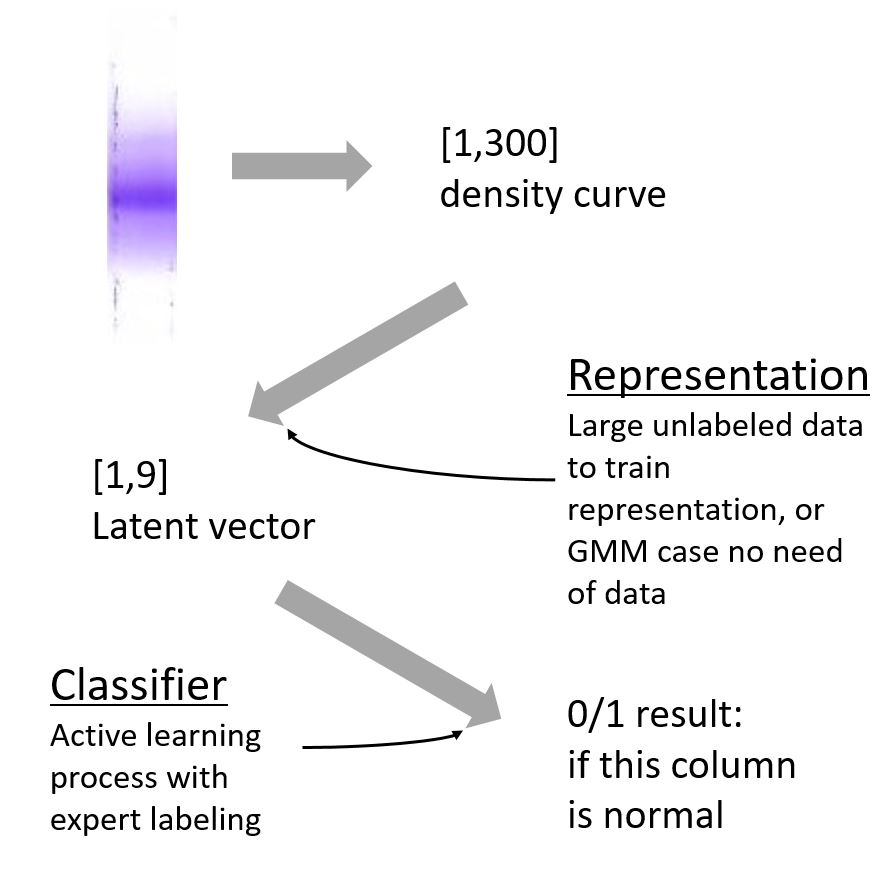
\includegraphics[width=0.8\linewidth]{fig_2.jpg}
    \end{center}
       \caption{Structure of the generative active learning framework}
    \end{figure}

\subsection{Choice of Generative Models}
Generative models in most cases are mapping functions from low-dimension prior of latent variables to high-dimension data space whose parameters maximises the likelihood of existing data\cite{goodfellow2016nips}. After training with adequate amount of data, we will have enough knowledge of all the decisive latent variables and we know exactly how these variables influence the corresponding point in data space. However, just generative is not enough. In testing state we need to encode all the test data to latent space. Hence, only bidirectional generative model are considered. Here, not only did we tried out classic bidirectional generative models including BiGAN and VAE, but we also hypothesized a GMM generative model using prior knowledge of the formation of IFE image. We can denote the decoder(generator) and encoder of the bidirectional model respectively as $D(z_i)$ and $E(x_i)$ so that we have $g(x_i)=f(E(x_i))$. Of course we expect that $D(E(x_i))$ to be as close as it can to $x_i$, or classifing $z_i$ will not provide any useful information.

\begin{figure}[t]
    \begin{center}
       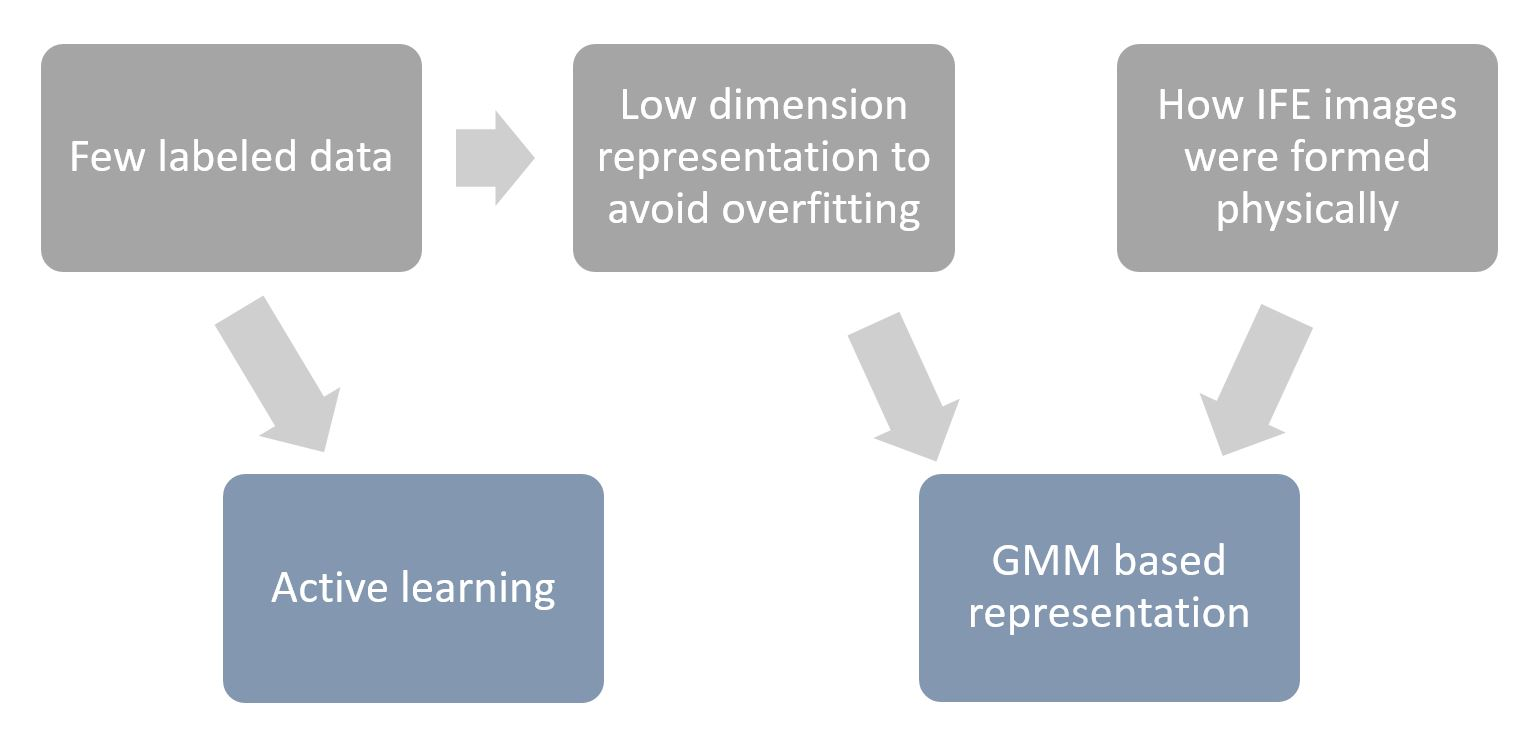
\includegraphics[width=0.8\linewidth]{motivation.jpg}
    \end{center}
       \caption{Motivation of our framework}
    \end{figure}

\subsubsection{GMM}
Gaussian mixture model is an iteritive aIgorithm using estimation maximization. It assumes that the data is the weighted conbination of several Gaussian distribution. The number of the components(Gaussian distribution) are usually set manually. Specifically, we can view the density plot of the gel electrophoresis as a sample, where the sample number of certain position is in direct proportion to the density of that position. Thus, ideally the density plot will be divide in to several seperate components of Gaussian distribution which approximates the concentration of charged protains(peaks). Choosing Gaussian mixture model to represent the formation of IFE image is not only natural, but also reasonable. For monoclonal band, the target Protein are all the same. Therefore if the electrophoresis procedure introduce no systematic error, all the monoclonal Protein should be in the same spot since the position that any type of Protein appears on the IFE image depends solely on its molecular properties such as weight and the electric charge it carries. In reality, noise is unavoidable, and we can suppose that the accumulation of small noises is under normal distribution. On the other hand, the polyclonal band can be perceived as a normal distribution whose mean (and variance) also obeys normal distribution becuase it contains many different kinds of Protein which have different weight and electric proterty. Every kind of Protein forms a normal distribution due to the noise of electrophoresis. Thus, it is still a normal distribution.%(can be proved, need to find prove or prove myself)
From above, we can derive that the one dimension signal is the empirical distrubution of the summation of several gaussian components. Empirically, in real data the number of gaussian components will not exceed 3.

In practice though, we use a variation of GMM which uses variational inference algorithms that do not need to suppose the number of gaussian components. The API called Bayesian Gaussian Mixture in sklearn\cite{scikit-learn}, and it is an infinite mixture model with the Dirichlet Process. In practice Dirichlet Process inference algorithm is approximated and uses a truncated distribution with a fixed maximum number of components (called the Stick-breaking representation). The number of components actually used almost always depends on the data\cite{article}\cite{ATTIAS2000A}. Thus we only need to fix the max number of Gaussian components, for example 3, and if only 2 of the components is working, than we will still get 3 components and one of them will have 0 weight.

\subsection{Hand Crafted Rules for GMM Vectors}
After we find the proper decomposition of the density plot(examples in section 3.2), we can use our prior knowledge to match peaks in different columns and determine if a peak indicates monoclonal component.
\par Firstly we try to preprocess the peak information provided by the GMM(Gaussian Mixture Model). GMM divide the density plot to several distinct Gaussian components, therefore it is possible that it may wrongly treat one polyclonal peak as the sum of two sharp(i.e. monoclonal) peaks. We can name the situation as "far overlap". For instance the 1 and 4 column in the figure 1.
\par However, a sharp peak in the middle of a polyclonal background is also a tricky problem. If the mean of the background peak and the sharp peak is almost the same, the GMM will give us unsatisfying result where the extracted sharp peak is not as sharp as we think. For instance column 5 in the figure 1. We can name this case "near overlap".
\par To sum up, the classification rules should be able to identify near and far overlap and of course stay robust when countering these cases. Identifying is easy because all we need to do is considering the means of every pair of components in one column for each column. Hence, the rule has two steps: preprocessing and classifying. In preprocessing step, we supress the far overlap components so that each one of them will be considered normal. Of course when the weight difference or the variance difference is too large this mechanism will not be trigered. At the same time, the weight of each peak of the near overlap case will be replaced by the sum of the weights. In the classifying step we can consider every components with the all the components in the rest of the columns, and the rules are similar with the peak detection method in the column matching part, but here we use $t=\frac{Variance}{n\_samples*weight}$ as the Identifying value. If t is lower than a manually set threshold than the classifier will lable it as abnormal.


\begin{figure}[t]
    \begin{center}
       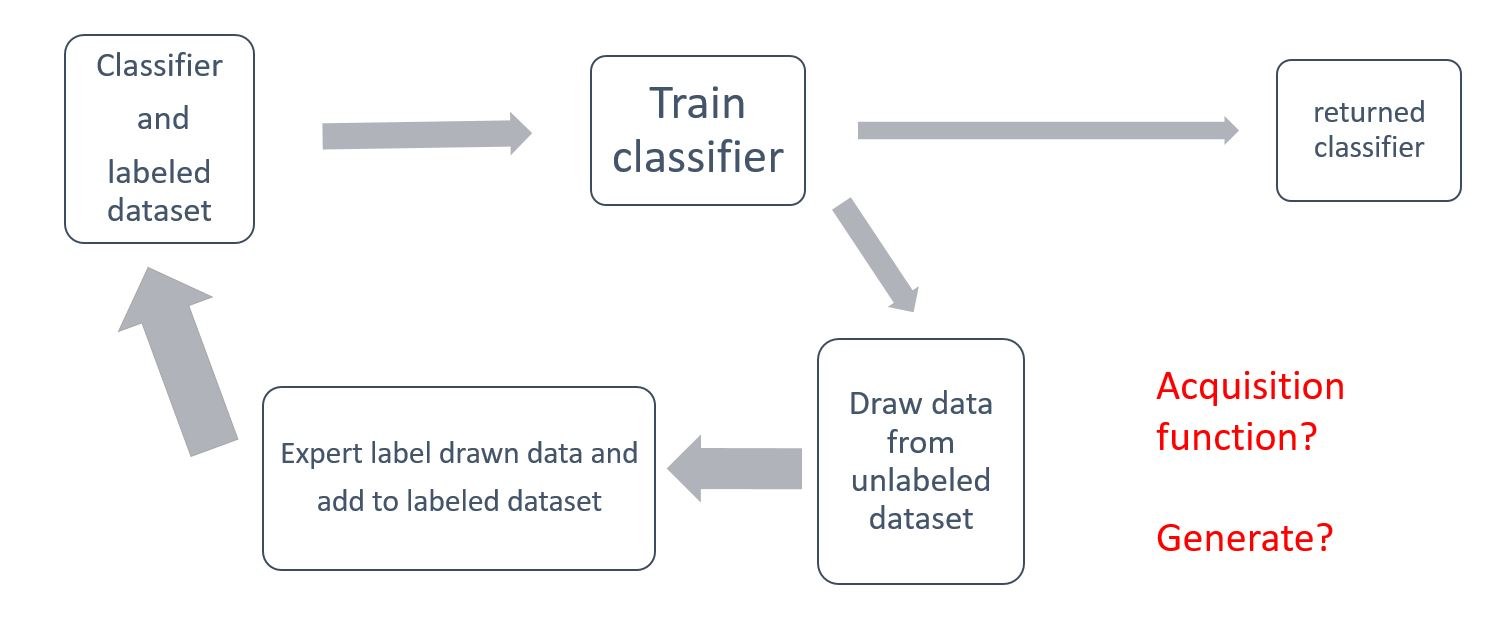
\includegraphics[width=0.8\linewidth]{active.jpg}
    \end{center}
       \caption{The iterative process of active leraning. We generate data samples to get more imformation}
    \end{figure}

\subsection{Active Learning Process}
After we completes the first stage of training process, we now have a low dimension embedding of the real data(300 dimension signal). The second stage is to actively train a classifier in this latent variable space. Each iteration of active learning contains the training of classifier, sampling data to be labeled, expert labeling and updating the training set. The main difference between generative active learning and traditional pool based active learning is the way of sampling. Here we can sample any point near the decision hyperplane because we can transform any point in latent space to a point in data space. According to the classifier, different sampling strategy can be used. For example, we conducted experiments on MNIST dataset and chose linear SVM as the classifier, we first choose 10 unknown data points from the pool that are nearest to the decision hyperplane of the linear SVM classifier, then we derive their projection on the decision hyperplane. This simple sampling method assures that the generated data points will be informative since they are in each iteration one of the most uncertain points in the latent space. As for the hand crafted rules' case, we aim to find the most informative data points to update the parameters in the rules(i.e. the $t$ from the above subsection and etc.) We can utilize reinforcement learning to update the parameters using labeled data, but combining reinforcement learning and active learning process is left for future research.

\section{Experiments}
To proof the concept of this framework, we performed experiments using this framework on not only the dataset of IFE images, but also the MNIST dataset.
\subsection{Different Representations(Generative Models) and Classifiers}
Different approaches to find the mapping between data space and latent space should be measured in several ways. For now, we compared all the combinations of different generative model and weak classifier in the latent space on 40 training data with label, 2000 synthesized data without label, and 20 testing data. We did not enable active learning in this comparative stage, so basically it is just a standard framework with feature extraction and classification. Plus, we constructed a comparative end to end neural network consists of VAE and MLP that can only utilizes the small labeled dataset. We aim to evaluate the performance of four representations: GMM, VAE, AE(auto-encoder), PCA(principle component analysis), four weak classifier: linear SVM, rbf SVM, decision tree, random forest. In addition, hand crafted rules including GMM rule and derivative filter are tested, and also the end to end neural network we mentioned.

\begin{table*}
    \centering
    \caption{Result of different combinations of representations and classifiers}
      \begin{tabular}{rcrrrrcc}
        \hline
             & rule based & \multicolumn{1}{c}{linear svm} & \multicolumn{1}{c}{rbf svm} & \multicolumn{1}{c}{decision tree} & \multicolumn{1}{c}{random forest} & \multicolumn{1}{p{6.5em}}{end to end} & derivative filter \\
            \hline
      GMM   & \multicolumn{1}{r}{0.925} & 0.7   & 0.705 & 0.68  & 0.69  & \multirow{4}[0]{*}{0.725} & \multirow{4}[0]{*}{0.92} \\
      VAE   & \multicolumn{1}{c}{\multirow{3}[0]{*}{N/A}} & 0.71  & 0.8   & 0.7   & 0.755 &       &  \\
      AE    &       & 0.725 & 0.82  & 0.72  & 0.705 &       &  \\
      PCA   &       & 0.775 & 0.84  & 0.8   & 0.805 &       &  \\
      \hline
      \end{tabular}%
    \label{tab:addlabel}%
  \end{table*}

\begin{table}
    \centering
    \caption{Reconstruction error}
      \begin{tabular}{cr}
        \hline
            & \multicolumn{1}{p{12.535em}}{reconstruction error} \\
            \hline
      GMM   & 1.031 \\
      VAE   & 10.33 \\
      AE    & 4.16 \\
      PCA   & 26.99 \\
      \hline
      \end{tabular}%
    \label{tab:addlabel}%
  \end{table}%
  

Firstly, reconstruction error is the most important property of a representation. In ideal case, the mapping should be injective. If not, the classifier in latent space will not be able to provide valid judgement in data space. Partly because of the lack of large unlabeled real dataset, GMM achieved overwhelming advantage compared to other representations. What's more, every feature in the GMM vector has its essential meaning, and we clearly know how the latent space stands for. However, when it comes to auto encoder and variational auto encoder we do not even know whether the corresponding point will move if we change one of the feature in the latent vector.

Secondly, the test accuracy of different combinations not only reveals the capability of the representation and classifier, it also evaluates their matching degree. For example, GMM works well with specifically designed rule-based method, but due to its highly non-linear space, linear svm will achieve bad results. For other classifiers like decision trees and rbf SVM, they often tend to overfit because of the small labeled dataset not to mention the end to end model that solely based on neural network. They all achieves 100$\%$ in the training set but low accuracy on the test set. The derivative filter applys simple edge detection methods for example the 1$^{st}$ and 2$^{nd}$ derivative, and here we use it as a baseline.

In conclusion, GMM based generative model and rule based classifier is the best match for this IFE dataset. However, we cannot solely depend on manually drafted rules. In other words we still need labeled data to improve its generalizability.

\subsection{Combining Active Learning with SVM}
We will first present the result regarding the MNIST dataset(binary case of 3 and 8) which we use to prove our concept. Although Huijser and Gemert have implemented a model with SVM classifier in the latent space\cite{huijser2017active}, we cannot directly follow their results, because when the decision hyperplane is not linear like the case of GMM space, the novel boundary method will not work. Thus in this experiment, unfortunately, we still have to generate a few imformative data points instend of a clever boundary line, even if we can use linear SVM in the auto encoder latent space. We simply chose auto encoder as the generative model that will bridge the gap between the data space and latent space. This will be trained on all the data in the training set. Afterwards, we randomly pick 1\textperthousand \ of the training set to be the initial labeled data, and perform 10 iterations of active learning. In each iteration 10 generated data points will be labeled by an oracle, and the SVM classifier will be updated. We will compare this setting with the same amount of randomly picked data using the same auto encoder. In this random setting, the auto encoder simply works as a method of dimensionality reduction, as we do not need to decode the generated data points in latent space back to data space. Figure 5 is the images of generated data points after decoding into data space. We can see that almost every image transformed to the real data space requires close scrutiny to distinguish 3 from 8. They are on the decision hyperplane of the classifier in every iteration, thus after transformation into the real data space, they ought to be on the edge as well. When compared to the random chosen data, they tend to yeild more information. Figure 6 and table 3 compares the learning efficiency between random sampling in the data pool and active generation. The reason why active generation achieves worse result is probably because the human introduced error of hand written digits. As can be seen from figure 5, some of the generated images are hard to tell whether they belong to 3 or 8. For another, there is only 12 initial data, and all other data in active learning setting are near to the real decision hyperplane. We may consider introducing some of the balancing data(augmenting the known data which is far from the decision hyperplane) to alleviate this problem.

\begin{figure}[t]
    \begin{center}
       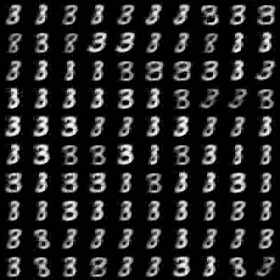
\includegraphics[width=0.8\linewidth]{active_process.png}
    \end{center}
       \caption{Generated pics in 10 iterations of active learning. Each row is an iteration.}
    \end{figure}

% Table generated by Excel2LaTeX from sheet 'Sheet1'
\begin{table*}
    \centering
    \caption{Compare between active learning and random pick}
      \begin{tabular}{lrrrrrrrrrrr}
        \hline
      data amount & 12    & 22    & 32    & 42    & 52    & 62    & 72    & 82    & 92    & 102   & 112 \\
      \hline
      active & 0.8594  & 0.8624  & 0.8624  & 0.8619  & 0.8619  & 0.8614  & 0.8614  & 0.8614  & 0.8619  & 0.8614  & 0.8609  \\
      random & 0.8594  & 0.8861  & 0.8866  & 0.8861  & 0.8876  & 0.8871  & 0.8876  & 0.8881  & 0.8881  & 0.8881  & 0.8881  \\
      \hline
      \end{tabular}%
    \label{tab:addlabel}%
  \end{table*}%
  
  

\subsection{Combining Active Learning with Rule Based Classifier}
Because of the active learning process, the embedding methods should satisfy the properties below. Data points that are close to each other will also have small distance in the latent space. Else the generated data points in latent space probably will not be imformative at all. In addition, GMM method is based on the formation process of IFE images, which endow it with great explainability. Thus it is natural to find out that using GMM as generative model, and the rule based classifier specifically designed for the latent vector produced by GMM model as the classifier model is the best combination for IFE image dataset.

\section{Conclusion}
To sum up, we have proposed an active learning framework that generates new data in order to achieve more information than traditional pool based methods. We applied this framework to a medical image dataset regarding with M-protain diagnostics and IFE. To achieve maximum use of our prior knowledge of the formation of an IFE image, we proposed a novel generative model specifically for this data set based on GMM, and constructed a rule based classifier which works in the latent space of GMM. We conducted extensive experiments to explore the best match of generative model and classifiers, including auto encoder, linear SVM on MNIST dataset and GMM, rule based classifier on IFE image dataset.


{\small
\bibliographystyle{ieee_fullname}
\bibliography{lib}
}

\end{document}
